\section{Goldstein-Price Function}
\label{sec:test_functions:goldstein_price}
  The \emph{Goldstein-Price function}, believed to be proposed by individuals
  named Goldstein and Price, is a challenging multimodal function recognized for
  its landscape densely populated with local minima.
  This function serves as a standard benchmark in the field of optimization,
  testing the efficacy of various algorithms.
  The precise origins of this function, however, remain elusive in academic
  literature.

  \begin{definition}[Goldstein-Price Function]
    \label{def:test_functions:goldstein_price}
      The \emph{Goldstein-Price function}, denoted as \(f: \mathbb{R}^2
      \rightarrow \mathbb{R}\), is formally articulated as follows:

      \begin{equation}
      \label{eq:test_functions:goldstein_price}
        \begin{split}
          f(x,\,y) = 
            & \left[
                1 + (x + y + 1)^2 
                  \cdot (19 - 14x + 3x^2 - 14y + 6xy + 3y^2) 
              \right] \\
            & \cdot \left[ 
                30 + (2x - 3y)^2 
                  \cdot (18 - 32x + 12x^2 + 48y - 36xy + 27y^2) 
              \right]
        \end{split}
      \end{equation}
  \end{definition}

  The function's global minimum is located at \(f(x^*,\,y^*) = 
  3\) with \((x^*,\,y^*) = (0,\,-1)\).
  Evaluations of the Goldstein-Price function are typically performed within the
  range \(x,\,y \in [-2,\, 2]\).

  \begin{figure}[ht!]
    \centering
    \begin{subfigure}[b]{0.45\textwidth}
      \centering
      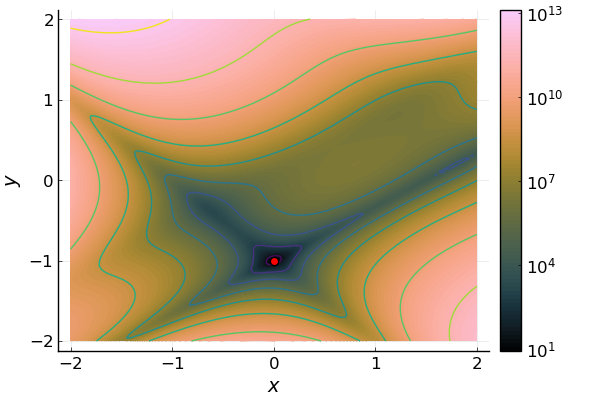
\includegraphics[width=\textwidth]
        {img/test_functions/goldstein_price_contour.png}
      \caption{Contour plot.}
      \label{fig:test_functions:goldstein_price:contour}
    \end{subfigure}
    \hfill
    \begin{subfigure}[b]{0.45\textwidth}
      \centering
      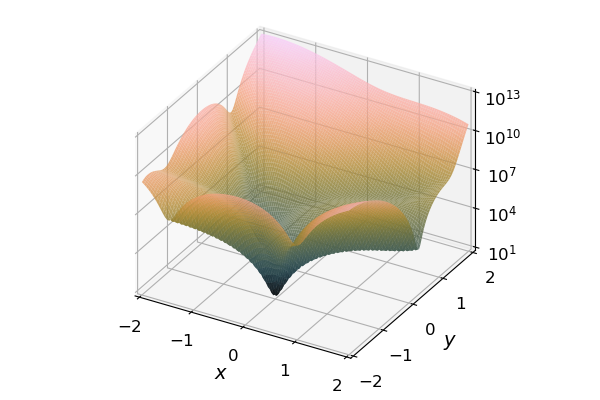
\includegraphics[width=\textwidth]
        {img/test_functions/goldstein_price_surface.png}
      \caption{Surface plot.}
      \label{fig:test_functions:goldstein_price:surface}
    \end{subfigure}
    \caption{Visual representations of the Goldstein-Price function}
    \label{fig:test_functions:goldstein_price}
  \end{figure}
